\section{Introduction}

Muon system is hosted in the steel yokes of the CMS detector~\cite{Chatrchyan:2008aa} and it is divided into a central part (barrel: $|\eta| < 1.2$) with Drift-Tube (DT) detectors and two forward parts (endcaps: $0.9 < |\eta| < 2.4$) with Cathode Strip Chambers (CSC) as shown in Fig.~\ref{fig:CMS_muon_system}. Resistive Plate Chambers (RPC) are located in barrel and endcap parts ($|\eta| < 1.9$). The detectors of the muon system identify muons, provide a fast muon trigger, and give a precise measurement of the muon trajectory. Performance of the CMS muon system in LHC Run1 is described in~\cite{Chatrchyan:2013sba}.

\begin{figure}[b]
        \begin{center}
                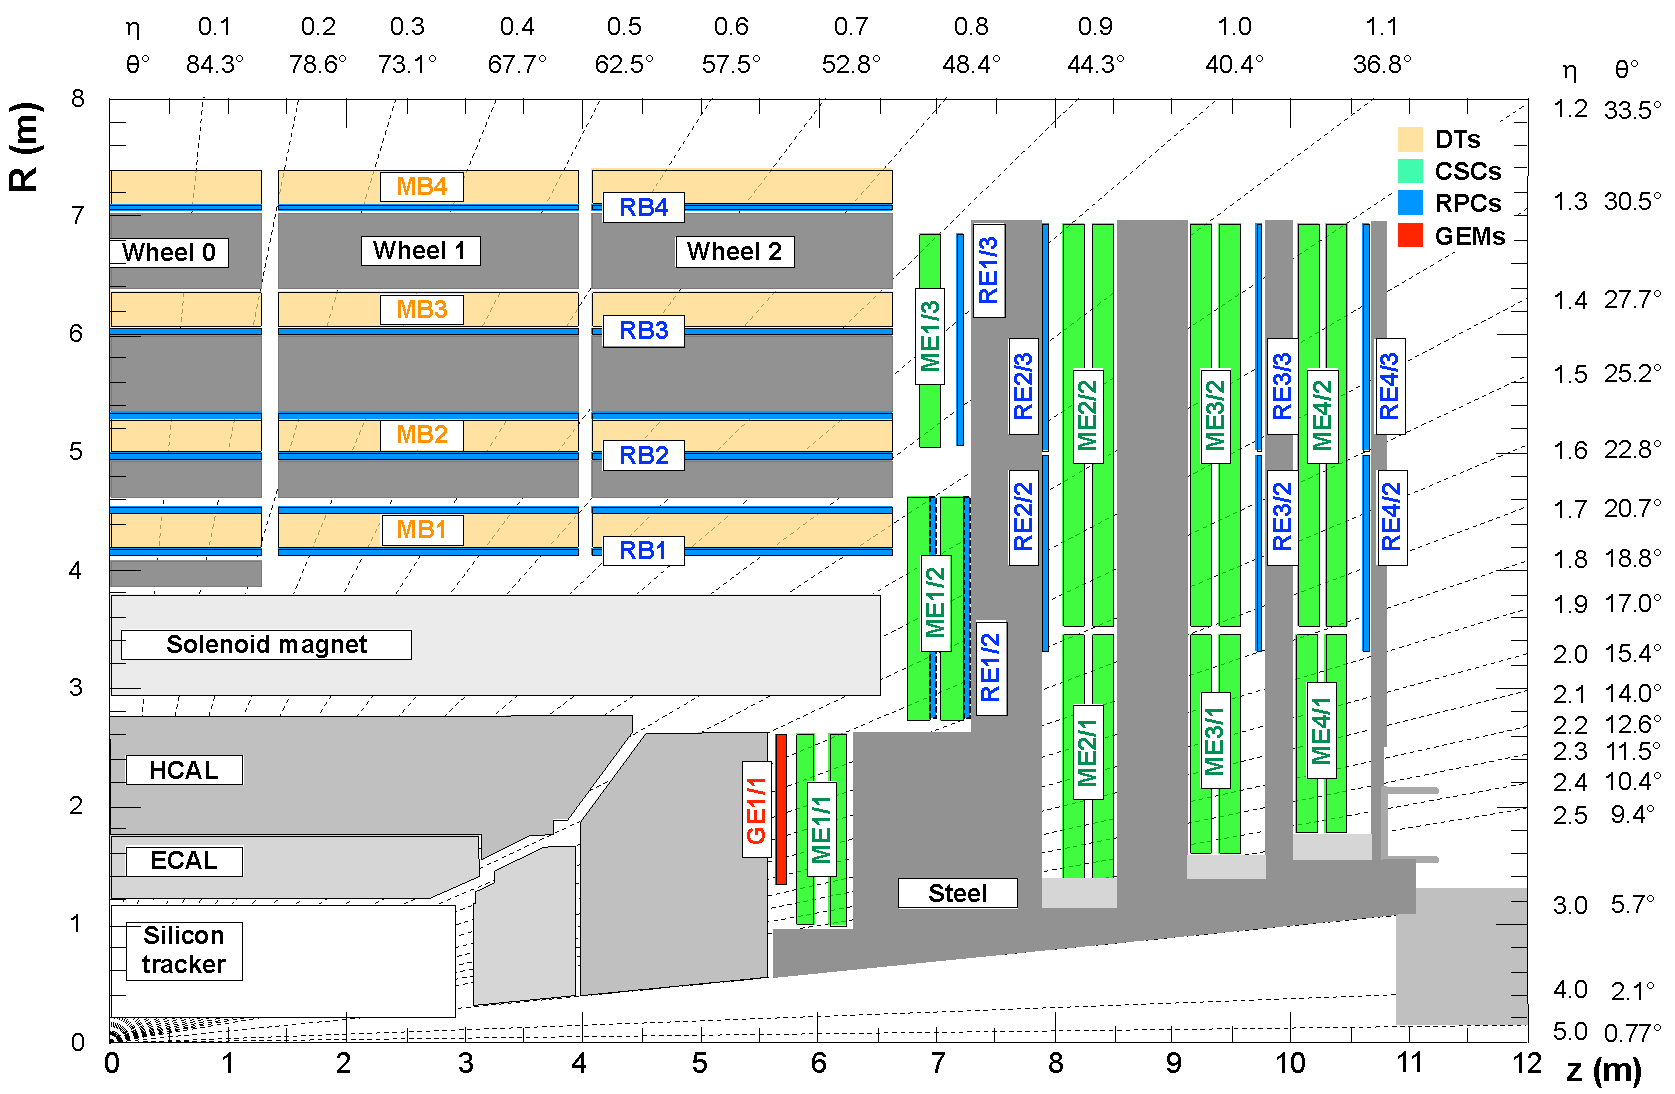
\includegraphics[width=0.99\linewidth]{figures/cms_upg_o_g_b_ni_ge11_r_grid_130919.pdf}
                \caption{Quarter-view of the CMS cross section. Detectors in the muon system are highlighted: DT -- orange, CSC -- green, RPC -- blue and future GE1/1 -- red.}
                \label{fig:CMS_muon_system}
        \end{center}
\end{figure}

The muon trigger is a tracking trigger that determines the momentum of muons using hits (position and angular measurements) in the muon system chambers situated in the magnetic field of the CMS detector. In this paper we describe several major improvements and upgrades to the muons system and their effect on the muon trigger performance. The focus of the muon trigger upgrade is to improve its rate reduction capability without significantly affecting the efficiency. We overview implementation of the muon trigger in endcaps in Section~\ref{sec:endcap_trigger}.

Installation of the outermost ring of CSCs in the fourth disk of each endcap (ME4/2) during 2013-2015 shutdown of the LHC (Long Shutdown 1 or LS1) allows to increase the number of muon hits along its trajectory. Major revision of the electronics for innermost ring of CSCs in the first disk (ME1/1) and unganging strips in the bottom part of these chambers allow to significantly enhance their performance in the trigger and in offline reconstruction. We describe details of the CSC upgrade during LS1 in Section~\ref{sec:csc_upgrade}.

New, robust and sophisticated, ME1/1 local trigger algorithm which is tolerant of the increased pile-up was also developed during LS1. Individual improvements of the upgraded algorithm are studied in details using simulation, and ranked in terms of their importance. The goal is to have improved ME1/1 local trigger algorithm commissioned during the 2015-16 Year-End Technical Stop (YETS), so that the upgraded trigger will be available to operate under high pile-up running conditions in 2016. Overview of the CSC local trigger algorithm is in Section~\ref{sec:csc_algo}. Specifics of the previous and upgraded algorithms implementation in electronics firmware, emulation in CMS software, as well as results of individual improvements are described in three sections:
\begin{enumerate}
\item anode signal processing (see Section~\ref{sec:alct}),
\item cathode signal processing (see Section~\ref{sec:clct}),
\item cathode-anode correlation (see Section~\ref{sec:lct}).
\end{enumerate}

As a part of future upgrade for Phase II of LHC running, the CMS will be equipped with Gas Electron Multiplier (GEM) detectors in the high pseudorapidity region ($1.5 < |\eta| < 2.2$) as shown in Fig.~\ref{fig:CMS_muon_system}. Pairs of triple-GEM chambers will be installed in the currently vacant position in front of the ME1/1 chambers and are dubbed GE1/1. The addition of such chambers allows to measure the bending angle of a track between GE1/1 and ME1/1. Usage of the bending angle at L1 can help to keep the rates down while having the efficiency high. Several implementation possibilities of the combined GEM-CSC local trigger algorithm for the high luminosity run of LHC are investigated in details in~\cite{CMS_DN-14-018}.